%!TEX root=../document.tex

\section{Ergebnisse}
\label{sec:Ergebnisse}

\subsection{Django-REST-Framework Tutorial}
Ich habe mit zur Bearbeitung dieser Übung die Django-REST-Schnittstelle ausgesucht.

\subsubsection{1: Proejtk Setup}
Zuerst muss ein neues Django Projekt erstellt und die Quickstart app aufgerufen werden.
Das Tutorial gibt hierbei vor, wie man über die Commandline ein Projekt erstellt und weitere Schritte. Diese haben jedoch nicht funktioniert, da das Command zum Erstellen eines neuen Projekts : \textbf{django-admin.py startproject tutorial .} keine Auswirkung hatte.

Lösung: Also wurde händisch über PyCharm ein neues Django Projekt angelegt und die Ordnerstruktur später manuell erweitert.

\subsubsection{Sync Database und Superuser}

Anschließend wird die Database über das Command \textbf{python manage.py migrate} zum ersten mal Angeglichen und ein neuer Superuser wird mit \textbf{python manage.py migrate} angelegt.

Dieser hat den Username \textbf{admin} und das Passwort \textbf{password123}.

  

\begin{figure}[!h]
	\begin{center}
		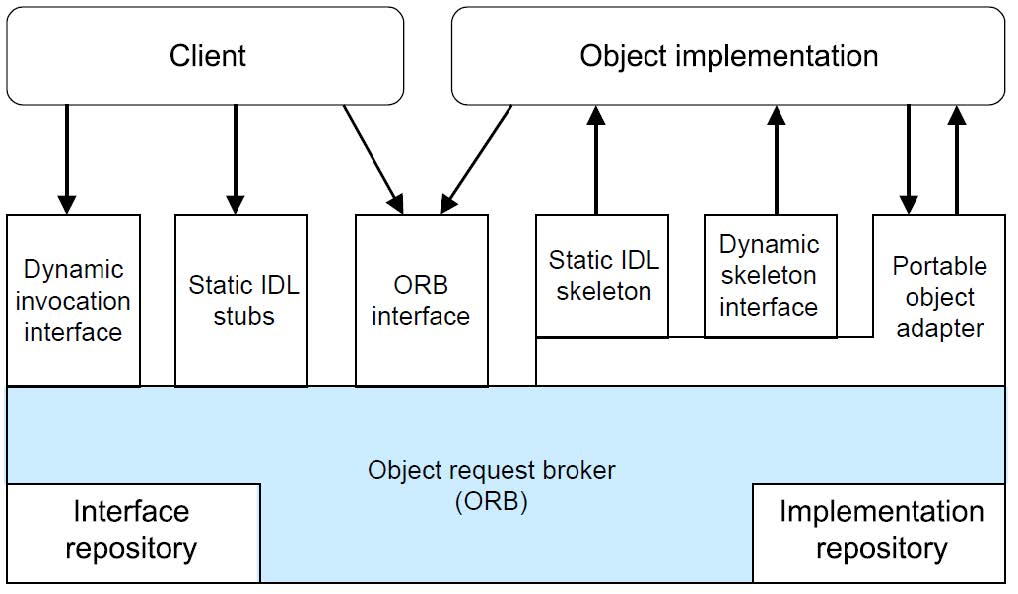
\includegraphics[width=0.5\linewidth]{images/corba.jpg}
		\caption{Common Object-Request-Broker Architecture \cite{tanenbaum2007verteilte}}
		\label{broker}
	\end{center}
\end{figure}

Hier sollen die Schritte der Laborübung erläutert werden. Alle Fragestellungen der Lehrkraft müssen hier beantwortet werden. Etwaige Probleme bzw. Schwierigkeiten sollten ebenfalls hier angeführt werden.

Es kann gut möglich sein, dass Lehrkräfte hier auch noch andere Eckpunkte explizit verlangen. Diese können dann in der selben Hierarchiestufe wie die \textit{\nameref{sec:Ergebnisse}} eingeordnet werden. Viel Spass nun mit einer kleinen Übersicht von \LaTeX-Elementen.

\subsection{Tabelle}
\renewcommand{\arraystretch}{1.5}
\begin{table}[!h]
	\center
	\begin{tabular}{ | @{\hspace{3mm}} c @{\hspace{3mm}} | @{\hspace{3mm}} l @{\hspace{3mm}} | }
		\hline Header & Kopf\\ \hline\hline
		\textbf{Lorem} & Ipsum dolor sit amet, consetetur sadipscing elitr\\ \hline
		\textbf{Ipsum} & At vero eos et accusam et justo duo dolores et ea rebum.\\
			& Stet clita kasd gubergren, no sea takimata sanctus\\ \hline
		\textbf{Dolor} & Consetetur sadipscing elitr, sed diam nonumy\\\hline
	\end{tabular}
	\caption{Lorem ipsum dolor sit amet \cite{tanenbaum2007verteilte}}
	\label{methoden}
\end{table}

\subsection{Aufzählung}

\begin{itemize}
	\item \textbf{Lorem ipsum:} dolor sit amet, consetetur sadipscing elitr
	\item sed diam nonumy eirmod tempor invidunt ut labore et dolore magna aliquyam erat
	\item ut labore et dolore magna aliquyam erat, sed diam voluptua
\end{itemize}

\subsection{Code}

At vero eos et accusam et justo duo dolores et ea rebum.

\begin{lstlisting}[style=Java, caption=Implizite Transaktion \cite{tanenbaum2007verteilte}]
try{
   gTransCur.begin();
   //Perform the operation inside the transaction
   not_registered = 
       gRegistrarObjRef.register_for_courses(student_id,selected_course_numbers);


   if (not_registered != null)

     //If operation executes with no errors, commit the transaction
     boolean report_heuristics = true;
     gTransCur.commit(report_heuristics);

   } else gTransCur.rollback();


} catch(org.omg.CosTransactions.NoTransaction nte) {
    System.err.println("NoTransaction: " + nte);
    System.exit(1);
} catch(org.omg.CosTransactions.SubtransactionsUnavailable e) {
    System.err.println("Subtransactions Unavailable: " + e);
    System.exit(1);
} catch(org.omg.CosTransactions.HeuristicHazard e) {
    System.err.println("HeuristicHazard: " + e);
    System.exit(1);
} catch(org.omg.CosTransactions.HeuristicMixed e) {
    System.err.println("HeuristicMixed: " + e);
    System.exit(1);
}
\end{lstlisting}

